\chapter{Ripetere} \label{cap:ripetere}

Nella presente versione 0.9.1, 31 agosto 2017, questo capitolo per il momento può essere consultato nella versione 0.4 del 9 settembre, reperibile all'indirizzo http://iamarf.ch/unifi/Piccolo-manuale-LibreLogo.pdf. In questa versione il capitolo si trova alle pagine 73-85.


\section{Cicli}

Introduciamo i cicli attraverso un piccolo studio geometrico. Riprendiamo il disegno di un quadrato, così come l'avevamo fatto nella sezione \ref{sec:comandi-fondamentali}\footnote{L'unica differenza rispetto al quadrato disegnato precedentemente è che qui, dopo avere disegnato il quarto lato, quello in basso, abbiamo lasciato la tartaruga lì, nel vertice in basso a sinistra, senza mandarla in alto, cosa che prima avevamo fatto per poter iniziare il disegno del tetto della casa.}.

\vskip 1cm

\begin{scriptsize}
\begin{minipage}{0.40\textwidth}
\begin{itemize}[itemsep=-3pt,parsep=2pt]
\item[] CLEARSCREEN          
\item[] HOME
\item[] FORWARD 50mm RIGHT 90
\item[] FORWARD 50mm RIGHT 90
\item[] FORWARD 50mm RIGHT 90
\item[] FORWARD 50mm RIGHT 90
\end{itemize}
\end{minipage}
\end{scriptsize}
\begin{minipage}{0.4\textwidth}
\begin{figure}[H]
   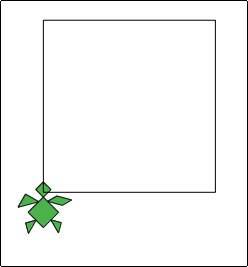
\includegraphics[width=3.0cm,trim=4 4 8 4,clip]{./images/ripetere/ripetere-1.png}
   \label{rip-1-a}
\end{figure}
\end{minipage} \hfill

\vskip 1cm

Modifichiamo questo codice usando le variabili, che avevamo visto nella sezione \ref{sec:variabili}. 

\vskip 1cm

\begin{scriptsize}
\begin{minipage}{0.40\textwidth}
\begin{itemize}[itemsep=-3pt,parsep=2pt]
\item[] CLEARSCREEN                                        
\item[] HOME
\item[] L = 50mm
\item[] A = 90
\item[] FORWARD L RIGHT A
\item[] FORWARD L RIGHT A
\item[] FORWARD L RIGHT A
\item[] FORWARD L RIGHT A                                  
\end{itemize}
\end{minipage}
\end{scriptsize}
\begin{minipage}{0.4\textwidth}
\begin{figure}[H]
   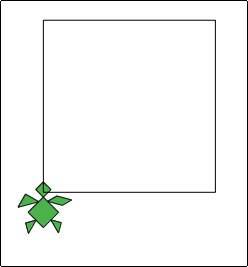
\includegraphics[width=3.0cm,trim=4 4 8 4,clip]{./images/ripetere/ripetere-1.png}
   \label{rip-2-a}
\end{figure}
\end{minipage} \hfill

dove L è il lato del quadrato e A l'angolo interno ad ogni vertice. È facile modificare questo codice per disegnare altre figure, e in particolare per disegnare poligoni regolari. Proviamo ad esempio a costruire un  triangolo equilatero. Come si potrebbe fare? Facile: si toglie un lato e si aggiusta la dimensione degli angoli interni. Per fare il quadrato la tartaruga doveva girare nello stesso verso quattro volte di un angolo di 90\degree, per un totale di 360\degree. Infatti dopo avere costruito, il quadrato la tartaruga punta nuovamente nella direzione iniziale: segno che ha fatto un giro completo, ovvero che ha ruotato complessivamente di 360\degree. La stessa cosa dovrà accadere con qualsiasi altra figura geometrica chiusa, quindi anche con un triangolo. Siccome abbiamo deciso di costruire poligoni regolari, tutti gli angoli interni dovranno essere uguali. E poiché un triangolo ha tre angoli interni, ciascuno di questi misurerà 120\degree = 360\degree/3:

\vskip 1cm

\begin{scriptsize}
\begin{minipage}{0.40\textwidth}
\begin{itemize}[itemsep=-3pt,parsep=2pt]
\item[] CLEARSCREEN          
\item[] HOME
\item[] L = 50mm
\item[] A = \textbf{120}	
\item[] FORWARD L RIGHT A
\item[] FORWARD L RIGHT A
\item[] FORWARD L RIGHT A
\end{itemize}
\end{minipage}
\end{scriptsize}
\begin{minipage}{0.4\textwidth}
\begin{figure}[H]
   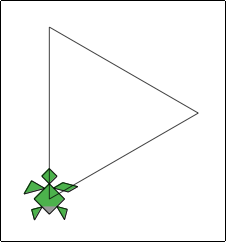
\includegraphics[width=3.0cm,trim=4 4 8 4,clip]{./images/ripetere/ripetere-2.png}
   \label{rip-1-b}
\end{figure}
\end{minipage} \hfill

\vskip 1cm

Proviamo invece ad aggiungere un lato. Invece di togliere dovremmo aggiungere un'istruzione \textbf{FORWARD L RIGHT A} alla versione che produce il quadrato, mentre per l'angolo dobbiamo calcolare 72\degree = 360\degree/5 e inserire questo valore nel codice. Ma fermiamoci un attimo a riflettere. Stiamo imparando a manovrare una “macchina” alla quale possiamo dare istruzioni affinché faccia delle cose al posto nostro. Perché quindi dobbiamo fare un calcolo per dare i dati necessari? Non potrebbe fare tutti i calcoli lei?  Non potremmo cambiare le cose in modo da darle le informazioni necessarie in modo più intuitivo? Lascio lo spazio qui sotto vuoto, se, tu lettore, vuoi rifletterci, prendere un appunto o provare da solo addirittura. Poi, quando vuoi, puoi passare alla pagina successiva.

\pagebreak

Procediamo allora introducendo la variabile \textbf{N} per designare il numero di lati  e poi facciamo calcolare al programma il valore dell'angolo:

\vskip 1cm

\begin{scriptsize}
\begin{minipage}{0.40\textwidth}
\begin{itemize}[itemsep=-3pt,parsep=2pt]
\item[] CLEARSCREEN                                 
\item[] HOME
\item[] L = 50mm
\item[] \textbf{N = 5}
\item[] \textbf{A = 360/N}
\item[] FORWARD L RIGHT A
\item[] FORWARD L RIGHT A
\item[] FORWARD L RIGHT A
\item[] FORWARD L RIGHT A
\item[] FORWARD L RIGHT A                           
\end{itemize}
\end{minipage}
\end{scriptsize}
\begin{minipage}{0.4\textwidth}
\begin{figure}[H]
   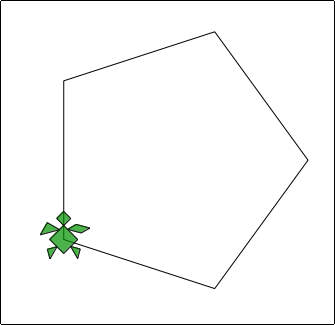
\includegraphics[width=3.0cm,trim=4 4 8 4,clip]{./images/ripetere/ripetere-3.png}
   \label{rip-2-b}
\end{figure}
\end{minipage} \hfill

dove L è il lato del poligono, N il numero di lati e A la misura degli angoli interni.

Sarà facile ora divertirsi a vedere come vengono poligoni con più lati. I calcoli li fa tutti il computer, si devono solo aggiungere istruzioni \textbf{FORWARD L RIGHT A}, tante quanti sono il numero dei lati: 3 per il triangolo equilatero, 4 per il quadrato, 5 per il pentagono, 6 per l'esagono e così via. Fino a quando? Finché ci pare, la matematica non pone limiti all'immaginazione. Ma la realtà sì: presto, andando avanti in una simile sperimentazione, incorreresti in un problema. In realtà ce ne possiamo accorgere anche solo guardando le  figure che abbiamo appena costruito. Cosa cambia, oltre al numero dei lati, passando dal poligono a 3 lati a quello a 4, e quindi a quello a 5? Prova a immaginare, oppure prova tu stesso in un documento nuovo, copiando il codice qui sopra e eseguendolo con diversi valori di N.

Vado a pagina nuova per lasciarti il tempo di pensare o provare.

\pagebreak

Quello che succede è che, aumentando il numero di lati aumenta la superficie della figura. È intuitivo: ogni volta si aggiunge un lato, quindi il perimetro aumenta. Poiché la figura è convessa\footnote{Detto in italiano, una figura è convessa se il suo perimetro non ha “bozze” verso l'interno.} la superficie non può che crescere, con l'aumentare del perimetro. Quindi, noi possiamo immaginare i poligoni che vogliamo ma se li costruiamo con il nostro codice presto usciranno dal foglio! Quindi che possiamo fare? Un'idea può essere quella di mantenere il perimetro costante. Questo significa che, se vogliamo generare figure con un numero sempre più grande di lati, dobbiamo anche diminuire progressivamente la lunghezza di questi affinché il perimetro rimanga costante. Ci occorre una regola, che è presto detta: in un poligono regolare il perimetro si può ottenere moltiplicando la lunghezza del lato per il numero di lati. Se il lato è lungo L e il numero di lati è N, allora il perimetro è P = L*N. Questa formula ci consente di fissare il perimetro P e il numero di lati L, ricavando la lunghezza del lato: L = P/N. Scateniamoci: disegniamo un decagono regolare (10 lati)  

\begin{scriptsize}
\begin{minipage}{0.40\textwidth}
\begin{itemize}[itemsep=-3pt,parsep=2pt]
\item[] CLEARSCREEN         
\item[] HOME
\item[] \textbf{P = 200mm}
\item[] \textbf{N = 10}	
\item[] \textbf{L = P/N}      
\item[] \textbf{A = 360/N}     
\item[] FORWARD L RIGHT A
\item[] FORWARD L RIGHT A
\item[] FORWARD L RIGHT A
\item[] FORWARD L RIGHT A
\item[] FORWARD L RIGHT A
\item[] FORWARD L RIGHT A
\item[] FORWARD L RIGHT A
\item[] FORWARD L RIGHT A
\item[] FORWARD L RIGHT A
\item[] FORWARD L RIGHT A      
\end{itemize}
\end{minipage}
\end{scriptsize}
\begin{minipage}{0.4\textwidth}
\begin{figure}[H]
   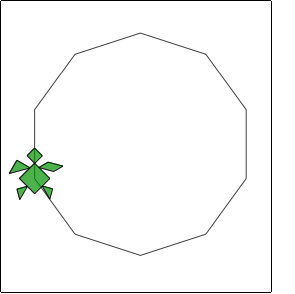
\includegraphics[width=3.0cm,trim=4 4 8 4,clip]{./images/ripetere/ripetere-4.png}
   \label{rip-3}
\end{figure}
\end{minipage} \hfill

Soddisfacente no? Anche perché così stiamo mettendo a frutto l'utilità delle variabili (sez. \ref{sec:variabili}), che forse alla prima non ci era parsa così chiara. Qui il fatto è evidente: possiamo inserire i dati numerici indispensabili e poi far calcolare i parametri derivati attraverso formule che utilizzano variabili simboliche. Una bella generalizzazione! Ma non siamo soddisfatti, a dire il vero. Infatti, per conseguire il nostro obiettivo di un un programma che disegni un poligono regolare qualsiasi siamo costretti a fare  una cosa “sporca”: ci tocca inserire a mano tante nuove istruzioni  \textbf{FORWARD L RIGHT A} quanti sono i lati. Funziona, ma non è “elegante”, e l'eleganza in matematica, come nella \textit{computer science}, non di rado si traduce in chiarezza, in maggiore facilità di risolvere problemi successivi. E qual è qui il nostro problema? Quello di dover riscrivere, o copia-incollare, più volte la stessa identica istruzione: qualcosa che stride con la bell'idea di immaginare poligoni regolari qualsivoglia... e qui vengono i “cicli”.

In tutti i linguaggi di programmazione esistono costrutti che consentono di ripetere più volte una stessa sequenza di istruzioni. Anzi, in tutti i linguaggi esistono più modi per ripetere sequenze di istruzioni, anche in LibreLogo! Qui, il costrutto più semplice è il seguente:
    
\begin{scriptsize}
\begin{minipage}{0.40\textwidth}
\begin{itemize}[itemsep=-3pt,parsep=2pt]
\item[] CLEARSCREEN                 
\item[] HOME
\item[] P = 200mm
\item[] N = 10
\item[] L = P/N
\item[] A = 360/N
\item[] \textbf{REPEAT N [}
\item[]  \hspace{0.5cm}	\textbf{FORWARD L RIGHT A}
\item[] \textbf{]}                           
\end{itemize}
\end{minipage}
\end{scriptsize}
\begin{minipage}{0.4\textwidth}
\begin{figure}[H]
   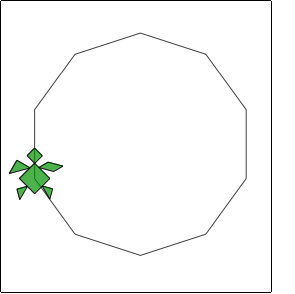
\includegraphics[width=3.0cm,trim=4 4 8 4,clip]{./images/ripetere/ripetere-4.png}
   \label{rip-4}
\end{figure}
\end{minipage} \hfill

\vskip 1cm

Abbiamo introdotto la novità brutalmente, all'interno di un problema, approfittando del fatto che in questo problema ci siamo già entrati (sperabilmente), e quindi confidando che il vantaggio sia più chiaro. I cicli in LibreLogo si possono realizzare con l'istruzione \textbf{REPEAT}, come nell'esempio precedente. Avremmo potuto anche scrivere \textbf{REPEAT 10 [ FORWARD 20 RIGHT 36 ]}: tutte le istruzioni che compaiono fra parentesi vengono ripetute tante volte quanto indicato dal numero dopo \textbf{REPEAT 10} in questo caso. Poiché “all'interno di un \textbf{REPEAT}” possono essere incluse anche mote istruzioni, queste possono essere anche incolonnate, scrivendo \textbf{REPEAT [} nella prima riga, ponendo le varie istruzioni da ripetere nelle righe sottostanti e scrivendo la parentesi quadra di chiusura \textbf{]} nell'ultima riga, come abbiamo fatto nell'esempio del decagono e nei successivi che seguono. In tutti questi esempi abbiamo anche usato le variabili, per indicare il numero di ripetizioni e gli argomenti degli spostamenti e dei mutamenti di direzione. Questo ci consente sperimentare il codice con parametri diversi, molto facilmente, per esempio per costruire poligoni con più lati. Vediamo per esempio come viene con 20 lati...

\begin{scriptsize}
\begin{minipage}{0.40\textwidth}
\begin{itemize}[itemsep=-3pt,parsep=2pt]
\item[] CLEARSCREEN                 
\item[] HOME
\item[] P = 200mm
\item[] N = 20
\item[] L = P/N
\item[] A = 360/N
\item[] \textbf{REPEAT N [}
\item[]  \hspace{0.5cm}	\textbf{FORWARD L RIGHT A}
\item[] \textbf{]}                           
\end{itemize}
\end{minipage}
\end{scriptsize}
\begin{minipage}{0.4\textwidth}
\begin{figure}[H]
   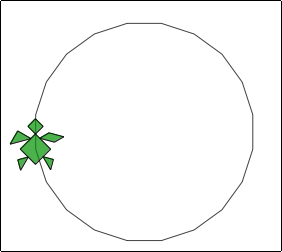
\includegraphics[width=3.0cm,trim=4 4 8 4,clip]{./images/ripetere/ripetere-5.png}
   \label{rip-5}
\end{figure}
\end{minipage} \hfill

\vskip 1cm

È anche evidente il vantaggio di scrivere in pochissime istruzioni un codice che senza il \textbf{REPEAT} ne richiederebbe moltissime. Si immagini qualcosa che si debba ripetere 100 o 1000 volte! 

Sarebbe interessante vedere la progressione dei poligoni regolari al crescere del numero di lati. 

\begin{centering}
\textit{Programming languages should have a “low floor” and a “high ceiling”}
\end{centering}

Questa frase viene attribuita a Seymour Papert: i linguaggi di programmazione dovrebbero avere un pavimento basso e un soffitto alto. Ovvero: devono essere facili per chi inizia ma poi non devono porre limiti. Logo, e naturalmente LibreLogo, è concepito per avviare al pensiero computazionale (e matematico) i più piccoli, ma può essere usato anche per obiettivi didattici molto più complessi. Il semplice codice che abbiamo creato contiene l'embrione di quella che potrebbe essere un'interessante e intuitiva introduzione dei concetti di infinito e infinitesimo, quando, nelle scuole secondarie di II grado si affrontano i limiti, le cui definizioni sono comprese, nella sostanza, da una percentuale piccolissima di studenti. Quei limiti che recuperano un po' di concretezza quando se ne imparano le prime applicazioni, per esempio attraverso il concetto di derivata. Ma tutto l'argomento resta, nella maggior parte dei casi, un territorio piuttosto ostile. Eppure è un territorio importantissimo – per coloro che si affacceranno allo studio della matematica e della fisica prenderà il nome di “analisi matematica”.  Ed è proprio dove appare l'infinito che la matematica si fa interessante e, perché no?, immaginifica. In fin dei conti la matematica è l'unico ambito dello scibile dove l'uomo, limitato in tutto e per tutto, riesce in qualche modo a mettere il guinzaglio all'infinito. Purtroppo, il primo contatto che gli studenti hanno con quello che potrebbe essere altrimenti una sorta di paese delle meraviglie, è disperatamente formale, racchiuso in diciture che finiscono per essere imparate a memoria senza lasciare alcuna traccia, che non sia un senso di frustrazione che si traduce nella consueta e ingiustificata consapevolezza di “non essere tagliati per la matematica”. L'esperienza concreta su come si possano disegnare dei poligoni regolari, toccando con mano il fatto che facendo crescere il numero di lati cresce il  perimetro, e constatando come invece si possa fare crescere indefinitamente tale numero rimpicciolendo i lati e lasciando così fermo il perimetro, potrebbe essere articolato in maniera da far scaturire i concetti di infinito e infinitesimo naturalmente e intuitivamente. Niente di formalmente rigoroso ma la comprensione dei concetti non scaturisce tanto dalle esposizioni formali quanto dall'associazione con concetti già noti. Nell'esempio che segue accenniamo a un percorso del genere, cogliendo l'occasione per aggiungere qualche particolare.

Proviamo quindi a disegnare una sequenza di poligoni regolari con un numero crescente di lati. Tu come faresti? L' esempio a pagina nuova.

\pagebreak

\begin{scriptsize}
\begin{minipage}{0.60\textwidth}
Per creare la successione di poligoni ricorriamo ad un ulteriore ciclo che contiene il precedente. Si parla in questo caso di “cicli annidati” (“nested cycles”). Oltre a questo, qui abbiamo fatto uso della variabile speciale REPCOUNT, che LibreLogo mette a disposizione come contatore delle ripetizioni di un ciclo.
\begin{itemize}[itemsep=-3pt,parsep=2pt]
\item[] CLEARSCREEN	; pulisco il foglio                            
\item[] HOME			; tartaruga a casa
\item[] 
\item[] PENUP		; alzo la penna
\item[] PENSIZE 2		; un tratto un po' più spesso
\item[] P = 50mm		; perimetro poligoni
\item[]                                                                  
\item[] REPEAT 10 [		; ciclo su 10 poligoni
\item[] 
\item[] ; Qui uso il  contatore dei cicli REPCOUNT
\item[] ; che parte da 1 e viene incrementato 
\item[] ; automaticamente di 1 a ogni ciclo.
\item[] ; Lo uso per calcolare il numero di lati N dei                   
\item[] ; poligoni, partendo da N = 3: quando
\item[] ; REPCOUNT vale 1 allora N deve valere 3
\item[] 
\item[] 	N = REPCOUNT+2
\item[] 	L = P/N	; lunghezza lato
\item[] 	A = 360/N	; ampiezza angolo                       
\item[] 
\item[] ; Qui uso il contatore REPCOUNT per fissare
\item[] ; la posizione di ciascun poligono, partendo
\item[] ; dall'alto verso il basso. Per comprendere il 
\item[] ; valore di questi numeri vedi pag. 29 e seg. 
\item[]                                                                  
\item[] 	POSITION [380, 110+(REPCOUNT-1)*70]
\item[] 	HEADING 0	; punto in all'inizio di ogni pol.
\item[] 	PENDOWN	; calo la penna
\item[] 
\item[] ;	Disegno il poligono
\item[]                                                                  
\item[] 	REPEAT N [	; ciclo sui lati del poligono
\item[] 		FORWARD L RIGHT A
\item[] 	]
\item[] 	PENUP	; alzo la penna
\item[] ]
\item[] HIDETURTLE                                                       
\end{itemize}
Proviamo ora a aggiungere un'altra colonna di poligoni, a fianco della precedente.
\end{minipage}
\end{scriptsize}
\begin{minipage}{0.2\textwidth}
\begin{figure}[H]
   
\includegraphics[width=1.0cm,trim=4 4 8 4,clip]{./images/ripetere/ripetere-6.png}
   \label{rip-6}
\end{figure}
\end{minipage} \hfill

\vskip 1cm


\pagebreak

\begin{scriptsize}
\begin{minipage}{0.50\textwidth}
Nel codice qui sotto abbiamo aggiunto un ulteriore ciclo che serve a ripetere una seconda colonna di poligoni. Qui abbiamo dovuto introdurre una variabile REPCOUNT2 per memorizzare il contatore del ciclo più esterno, perché quando siamo all'interno del ciclo sui poligoni, per determinare la posizione di ciascuno di essi, abbiamo bisogno di ambedue i contatori. 

Un'altra novità è costituita dal carattere ~ (si chiama tilde) che in LibreLogo consente di interrompere un'istruzione e continuarla nella riga seguente.
\begin{itemize}[itemsep=-3pt,parsep=2pt, leftmargin=-0.0mm ]
\item[] CLEARSCREEN                                                    
\item[] HOME
\item[] PENUP
\item[] PENSIZE 2
\item[] P = 50mm
\item[] NP = 8
\item[] PENUP                                                           
\item[] 
\item[] REPEAT 2 [			; ciclo sulle colonne
\item[] 
\item[] ; memorizzo in REPCOUNT2 il contatore del ciclo
\item[] ; esterno sulle colonne di poligoni
\item[]                                                                 
\item[] 	REPCOUNT2 =REPCOUNT
\item[] 	REPEAT NP [		; ciclo sui poligoni
\item[] 		N = (REPCOUNT2-1)*NP+REPCOUNT+2
\item[] 		L = P/N
\item[] 		A = 360/N
\item[] 		POSITION [380+(REPCOUNT2-1)*70, ~
\item[] 			110+(REPCOUNT-1)*70 ~
\item[] 			-(REPCOUNT2-1)*5]
\item[] 		HEADING 0
\item[] 		PENDOWN
\item[] 		REPEAT N [	; ciclo sui lati del poligono
\item[] 			FORWARD L RIGHT A                       
\item[] 		]
\item[] 		PENUP
\item[] 	]
\item[] ]
\item[] HIDETURTLE                                                     
\end{itemize}
\end{minipage}
\end{scriptsize}
\begin{minipage}{0.3\textwidth}
\begin{figure}[H]
   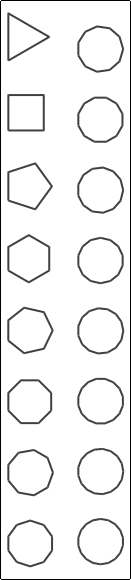
\includegraphics[width=2.5cm,trim=4 4 8 4,clip]{./images/ripetere/ripetere-7.png}
   \label{rip-7}
\end{figure}
\end{minipage} \hfill

\vskip 1cm

\pagebreak

Così, disegnando poligoni, ci troviamo nei pressi del cerchio, che può essere visto in una luce nuova: come un poligono che ha infiniti lati infinitamente piccini. Conducendo pazientemente gli studenti in un'esercitazione del genere si potrebbero fare varie considerazioni interessanti.
Un'osservazione sulla scrittura del codice. Negli esempi precedenti abbiamo incolonnato le istruzioni in maniera particolare, usando la tabulazione (rientro, indenting) così da mettere in evidenza i diversi cicli:  una tabulazione per le istruzioni nel ciclo più esterno (\textbf{REPEAT 2}), due tabulazioni nel ciclo sui poligoni (\textbf{REPEAT NP}) e tre tabulazioni nel ciclo più interno sui lati di ogni poligono (\textbf{REPEAT N}). In questo modo la struttura del codice è subito chiara. La presenza delle tabulazioni non influenza in alcun modo la funzionalità del programma in LibreLogo, serve solo a facilitare la leggibilità del codice. Non è sempre così con gli altri linguaggi di programmazione. Per esempio con il linguaggio Python la tabulazione influenza il comportamento del codice. In generale, è comunque molto importante scrivere il codice in modo chiaro e ordinato, intercalando i blocchi di codice con spazi, commenti e usando le tabulazioni.
L'istruzione \textbf{REPEAT} può essere usata anche senza l'argomento che specifica il numero dei cicli, ad esempio si potrebbe scrivere \textbf{REPEAT [ FORWARD 100 RIGHT 90 ]}. In questo modo quello che si ottiene è un quadrato ma in realtà il programma rimane apparentemente bloccato, senza che si riesca più ad agire sul documento. Dico apparentemente perché quello che in realtà succede è che la tartaruga continua a disegnare il contorno del quadrato infinite volte. Infatti, se non si specifica il numero di cicli dopo \textbf{REPEAT}, il programma continua a ripetere cicli all'infinito! Se succede una cosa del genere si deve agire mediante il tasto di stop
\includegraphics[height=1em]{./images/ripetere/StopLO.png}   per recuperare il controllo del documento. Questo è un fatto interessante che getta un po' di luce su quelle circostanze che spesso vengono confinate nell'idea che il computer “si  è bloccato”. In realtà spesso non si è affatto bloccato ma lavora alacremente, magari, come in questo caso, ripetendo una stessa sequenza di operazioni all'infinito oppure per un numero molto grande di volte. Si tratta di condizioni particolari, che facilmente dipendono da comportamenti scorretti dell'utente (per esempio per avere aperto troppi processi: finestre) o da errori di programmazione (bug) di chi ha scritto il software.
Oltre a \textbf{REPEAT} esistono altre istruzioni per eseguire i cicli ma richiedono la conoscenza di costrutti che dobbiamo ancora affrontare. 

\subsection{Operazioni aritmetiche}

Negli esempi precedenti, un po' in sordina, insieme alle variabili abbiamo introdotto le operazioni aritmetiche: la tartaruga disegna ma sa anche fare calcoli. Ecco le operazioni aritmetiche che si possono fare in  LibreLogo:

\begin{center}
%\begin{tabular}{| >{\centering\arraybackslash}m{1in} | >{\centering\arraybackslash}m{1in} |}
\begin{tabular}{| c | c | c |}
\hline
+ & 	Somma 			& 	10+3=13 		\\ \hline
- & 	Sottrazione 		& 	10-3=7	 		\\ \hline
* & 	Moltiplicazione 	&	10*3=30 		\\ \hline
/ & 	Divisione 		& 	10/3=3.$\overline{3}$ 	\\ \hline
// & 	Quoziente (intero) 	& 	10//3=3 		\\ \hline
\% & 	Resto (modulo) 		& 	10\%3=1 		\\ \hline
** & 	Elevamento a potenza 	& 	10**3=1000 		\\ \hline
\end{tabular}
\end{center}

È possibile un impiego marginale interessante: se si sta scrivendo un documento qaulasiasi in Writer, e LibreLogo è attivo, volendo si ha disposizione anche una calcolatrice. Con l'occasione, anticipiamo l'istruzione \textbf{LABEL “pippo”} che  scrive il testo “pippo” nel punto in cui si trova la tartaruga. Se invece si ha una variabile, per esempo di nome A, e se ne vuole scrivere il contenuto nel documento, allora baasta eseguire \textbf{LABEL A} A. Bene, facciamo ora un esempio di uso di LibreLogo come calcolatrice. Supponiamo che si voglia calcolare il 21\% di 127. Si scrive il seguente pezzetto di codice...
A = 127
B = 21
LABEL B/A*100

e lo si esegue: la tartaruga scrive  16.535433070866144. Bene, il risultato è 16.5\%. Da questo possiamo prendere il numero di decimali che ci fa comodo. Vedremo in seguito come troncare i decimali in LibreLogo o fare altre operazioni, anche molto più sofisticate. 

\subsection{Un accorgimento per trovare gli errori – la tartaruga troppo veloce!}

Non capita mai di scrivere il codice senza errori. Nello sviluppo di un software occorre sempre conteggiare anche il tempo necessario per individuare togliere gli errori. È sempre un'operazione onerosa e per ripulire veramente un software da tutti gli errori possono occorrere anni, con un processo di comunicazione continua fra chi ha scritto il software e chi lo usa. Si deve ovviamente cercare di pensare bene prima e evitare di commettere errori ma poi è normale commetterli. In gergo un errore si chiama “bug” (baco) e l'operazione di ricerca e correzione si chiama “debugging”. Le tecniche di debugging sono molto varie e anche molto sofisticate. Nel caso di LibreLogo, che produce grafica, può essere utile seguire attentamente il percorso fatto dalla tartaruga, che magari non è affatto quello che ci eravamo prefigurati. In primo luogo è utile rendere visibile la tartaruga, anche perché così, oltre a seguirla meglio con lo sguardo, si rallenta un po' il disegno. Tuttavia può non bastare e, se il disegno è troppo intricato, è facile perderne le tracce. Ebbene, qui torna utile l'istruzione \textbf{SLEEP}, che si usa con un argomento che dice per quanto tempo la tartaruga deve dormire (to sleep in inglese significa dormire). Questo tempo deve essere espresso in millisecondi (msec), quindi se scrivo \textbf{SLEEP 1000}, la tartaruga se ne sta ferma per 1000 msec, ovvero per un secondo. Si tratta quindi semplicemente di piazzare delle istruzioni SLEEP 1000 qua e là, in maniera da rallentare adeguatamente il disegno. Ho scritto 1000 ma è un valore indicativo. Occorre andare un po' per tentativi perché dipende dalla velocità del computer, da quante altre cose sta facendo e dalla complicazione del disegno. 

\subsection{Esercizi}

Può convenire cimentarsi in qualche esercizio, prima di andare avanti. Una soluzione degli esercizi può essere richiesta al sottoscritto: arf@unifi.it. Si faccia caso che ho scritto “una soluzione”. Questa è una caratteristica del i\textit{coding} da tenere ben presente: lo stesso risultato si può ottenere sempre in molti modi diversi.

\begin{minipage}{0.40\textwidth}
Si provi a riprodurre questo disegno utilizzando i cicli:                         
\end{minipage}
\begin{minipage}{0.4\textwidth}
\begin{figure}[H]
   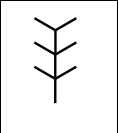
\includegraphics[width=3.0cm,trim=4 4 8 4,clip]{./images/ripetere/ripetere-8.png}
   \label{rip-8}
\end{figure}
\end{minipage} \hfill

\vskip 1cm


\begin{minipage}{0.40\textwidth}
Si provi quindi a costruire questo fiocco di neve:
\end{minipage}
\begin{minipage}{0.4\textwidth}
\begin{figure}[H]
   
\includegraphics[width=3.0cm,trim=4 4 8 4,clip]{./images/ripetere/ripetere-9.png}
   \label{rip-9}
\end{figure}
\end{minipage} \hfill


\vskip 1cm

\begin{minipage}{0.40\textwidth}
E se da questo fiocco tirassimo fuori una stella? 
\end{minipage}
\begin{minipage}{0.4\textwidth}
\begin{figure}[H]
   
\includegraphics[width=3.0cm,trim=4 4 8 4,clip]{./images/ripetere/ripetere-10.png}
   \label{rip-10}
\end{figure}
\end{minipage} \hfill

\vskip 1cm

\begin{minipage}{0.40\textwidth}
Naturale che sia venuta a 6 punte... ma se la volessimo a 7 punte? 
\end{minipage}
\begin{minipage}{0.4\textwidth}
\begin{figure}[H]
   
\includegraphics[width=3.0cm,trim=4 4 8 4,clip]{./images/ripetere/ripetere-11.png}
   \label{rip-11}
\end{figure}
\end{minipage} \hfill

\vskip 1cm

\begin{minipage}{0.40\textwidth}
Proviamo a sperimentare l'uso di un'operazione all'interno del \textbf{REPEAT}, per esempio per fare una spirale quadrata: 
\end{minipage}
\begin{minipage}{0.4\textwidth}
\begin{figure}[H]
   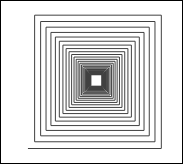
\includegraphics[width=3.0cm,trim=4 4 8 4,clip]{./images/ripetere/ripetere-12.png}
   \label{rip-12}
\end{figure}
\end{minipage} \hfill

\vskip 1cm

\begin{minipage}{0.40\textwidth}
Oppure un esercizio di frazioni: in modo per esempio che, dati il numeratore $N$ e il denominatore $M$, venga rappresentata la frazione $N/M$ con una torta:
\end{minipage}
\begin{minipage}{0.4\textwidth}
\begin{figure}[H]
   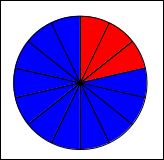
\includegraphics[width=3.0cm,trim=4 4 8 4,clip]{./images/ripetere/ripetere-13.png}
   \label{rip-13}
\end{figure}
\end{minipage} \hfill

E a proposito di \textit{low floor} and a \textit{high ceiling}, un esercizio  po' più difficile: disegnare un parallelepipedo in prospettiva, date le coordinate dei punti di fuga. Potrebbe andare bene per ragazzi di secondaria superiore (intersezione fra rette).

\vskip 1cm

\begin{figure}[H]
   \centering
   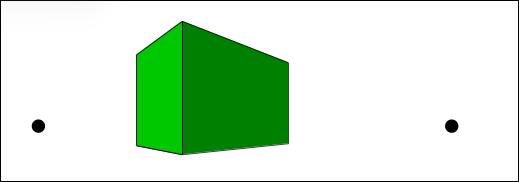
\includegraphics[width=10.0cm,trim=4 4 8 4,clip]{./images/ripetere/ripetere-14.png}
   \label{rip-14}
\end{figure}

\vskip 1cm
lll
\begin{figure}[H]
   \centering
   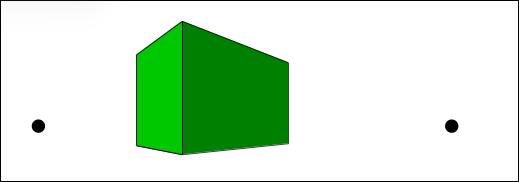
\includegraphics[width=10.0cm,trim=4 4 8 4,clip]{./images/ripetere/ripetere-14.png}
   \label{rip-15}
\end{figure}


